\section{Stromrichterschaltung}
\subsection{Gruppierung}
\subsubsection{nach Steuerung}
\begin{itemize}
    \item Ungesteuerte Stromrichter:
        \subitem Das Verhältnis von Eingangs- zu Ausgangsspannung wird durch die Stromrichterschaltung festgesetzt
    \item Gesteuerte Stromrichter
        \subitem Das Verhältnis von Eingangs- zu Ausgangsspannung wird durch Steuereingriff am Halbleiterschalter verändert. 
\end{itemize}

\subsubsection{nach Führung}
\textbf{Link:} \href{https://de.wikipedia.org/wiki/Kommutierung}{Kommutierung WIKI}\\[0.2cm]
\begin{minipage}{0.6\linewidth}
Kommutierung bedeutet die Wechslung des Stromflusses von einem HL-Ventil auf ein Anderes.
\begin{itemize}
    \item Netzgeführte Schaltung
        \subitem Kommutierungsspannung vom Netzwerk
    \item Lastgeführte Schaltung
        \subitem Kommutierungsspannung wird durch Lastkreis\\
        (z.B. Synchronmotor) gesteuert
    \item Selbstgeführte Schaltung
        \subitem Kommutierungsspannung wird selbst erzeugt
\end{itemize}
\end{minipage}
\begin{minipage}{0.4\linewidth}
    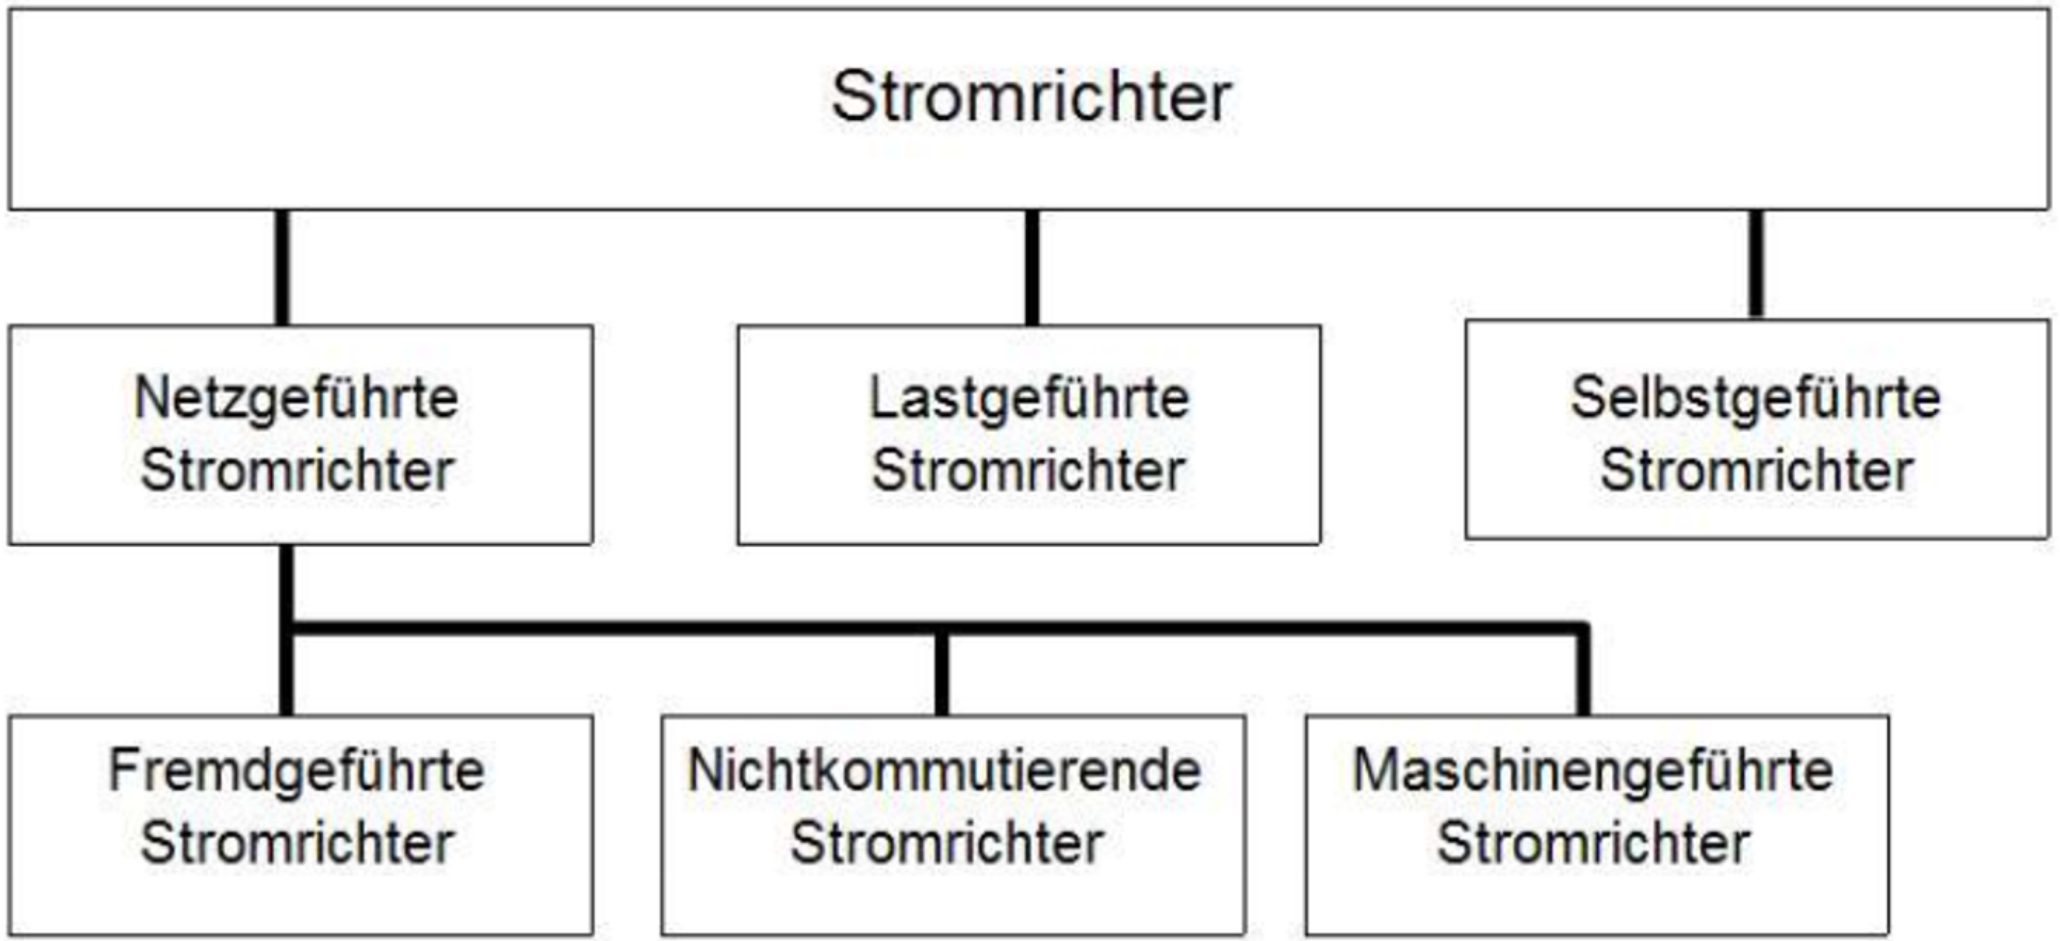
\includegraphics[width=\linewidth]{images/StromrichterKennzeichnung}\newline
\end{minipage}

\subsection{Kennzeichnung}
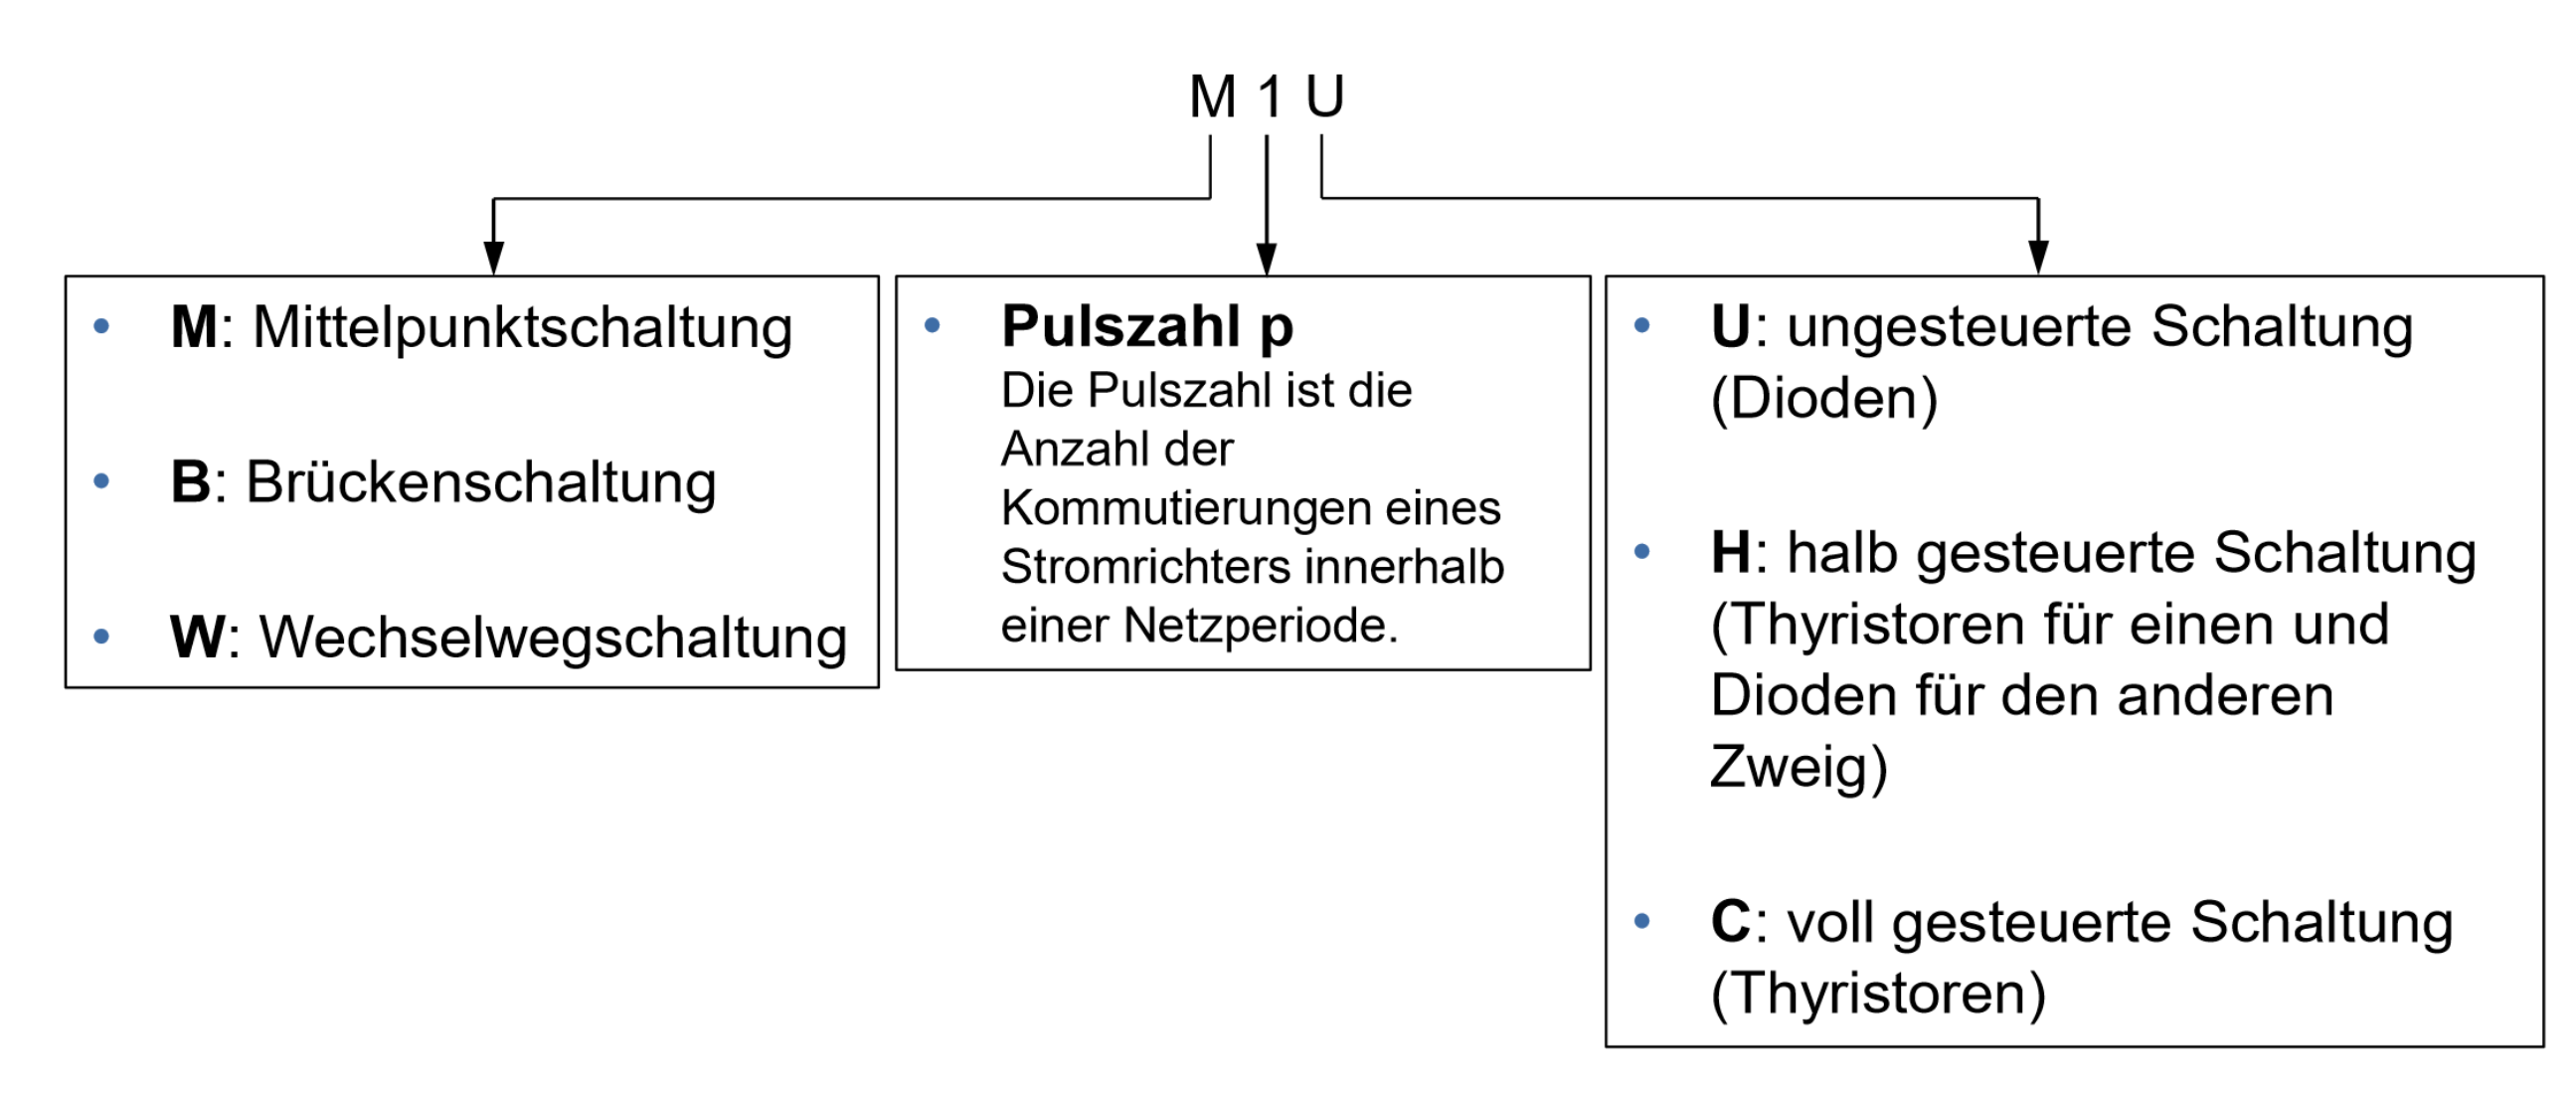
\includegraphics[width=\linewidth]{images/SRKennzeichnung}\newline
\href{https://de.wikipedia.org/wiki/Gleichrichter}{Gleichrichter WIKI}

%===================================================================
\clearpage